\documentclass[twoside]{book}

% Packages required by doxygen
\usepackage{fixltx2e}
\usepackage{calc}
\usepackage{doxygen}
\usepackage[export]{adjustbox} % also loads graphicx
\usepackage{graphicx}
\usepackage[utf8]{inputenc}
\usepackage{makeidx}
\usepackage{multicol}
\usepackage{multirow}
\PassOptionsToPackage{warn}{textcomp}
\usepackage{textcomp}
\usepackage[nointegrals]{wasysym}
\usepackage[table]{xcolor}

% Font selection
\usepackage[T1]{fontenc}
\usepackage[scaled=.90]{helvet}
\usepackage{courier}
\usepackage{amssymb}
\usepackage{sectsty}
\renewcommand{\familydefault}{\sfdefault}
\allsectionsfont{%
  \fontseries{bc}\selectfont%
  \color{darkgray}%
}
\renewcommand{\DoxyLabelFont}{%
  \fontseries{bc}\selectfont%
  \color{darkgray}%
}
\newcommand{\+}{\discretionary{\mbox{\scriptsize$\hookleftarrow$}}{}{}}

% Page & text layout
\usepackage{geometry}
\geometry{%
  a4paper,%
  top=2.5cm,%
  bottom=2.5cm,%
  left=2.5cm,%
  right=2.5cm%
}
\tolerance=750
\hfuzz=15pt
\hbadness=750
\setlength{\emergencystretch}{15pt}
\setlength{\parindent}{0cm}
\setlength{\parskip}{3ex plus 2ex minus 2ex}
\makeatletter
\renewcommand{\paragraph}{%
  \@startsection{paragraph}{4}{0ex}{-1.0ex}{1.0ex}{%
    \normalfont\normalsize\bfseries\SS@parafont%
  }%
}
\renewcommand{\subparagraph}{%
  \@startsection{subparagraph}{5}{0ex}{-1.0ex}{1.0ex}{%
    \normalfont\normalsize\bfseries\SS@subparafont%
  }%
}
\makeatother

% Headers & footers
\usepackage{fancyhdr}
\pagestyle{fancyplain}
\fancyhead[LE]{\fancyplain{}{\bfseries\thepage}}
\fancyhead[CE]{\fancyplain{}{}}
\fancyhead[RE]{\fancyplain{}{\bfseries\leftmark}}
\fancyhead[LO]{\fancyplain{}{\bfseries\rightmark}}
\fancyhead[CO]{\fancyplain{}{}}
\fancyhead[RO]{\fancyplain{}{\bfseries\thepage}}
\fancyfoot[LE]{\fancyplain{}{}}
\fancyfoot[CE]{\fancyplain{}{}}
\fancyfoot[RE]{\fancyplain{}{\bfseries\scriptsize Generated by Doxygen }}
\fancyfoot[LO]{\fancyplain{}{\bfseries\scriptsize Generated by Doxygen }}
\fancyfoot[CO]{\fancyplain{}{}}
\fancyfoot[RO]{\fancyplain{}{}}
\renewcommand{\footrulewidth}{0.4pt}
\renewcommand{\chaptermark}[1]{%
  \markboth{#1}{}%
}
\renewcommand{\sectionmark}[1]{%
  \markright{\thesection\ #1}%
}

% Indices & bibliography
\usepackage{natbib}
\usepackage[titles]{tocloft}
\setcounter{tocdepth}{3}
\setcounter{secnumdepth}{5}
\makeindex

% Hyperlinks (required, but should be loaded last)
\usepackage{ifpdf}
\ifpdf
  \usepackage[pdftex,pagebackref=true]{hyperref}
\else
  \usepackage[ps2pdf,pagebackref=true]{hyperref}
\fi
\hypersetup{%
  colorlinks=true,%
  linkcolor=blue,%
  citecolor=blue,%
  unicode%
}

% Custom commands
\newcommand{\clearemptydoublepage}{%
  \newpage{\pagestyle{empty}\cleardoublepage}%
}

\usepackage{caption}
\captionsetup{labelsep=space,justification=centering,font={bf},singlelinecheck=off,skip=4pt,position=top}

%===== C O N T E N T S =====

\begin{document}

% Titlepage & ToC
\hypersetup{pageanchor=false,
             bookmarksnumbered=true,
             pdfencoding=unicode
            }
\pagenumbering{alph}
\begin{titlepage}
\vspace*{7cm}
\begin{center}%
{\Large blueprint\+\_\+subsea\+\_\+oculus\+\_\+driver }\\
\vspace*{1cm}
{\large Generated by Doxygen 1.8.13}\\
\end{center}
\end{titlepage}
\clearemptydoublepage
\pagenumbering{roman}
\tableofcontents
\clearemptydoublepage
\pagenumbering{arabic}
\hypersetup{pageanchor=true}

%--- Begin generated contents ---
\chapter{Class Index}
\section{Class List}
Here are the classes, structs, unions and interfaces with brief descriptions\+:\begin{DoxyCompactList}
\item\contentsline{section}{\hyperlink{structOculusDriver_1_1DataPacket}{Oculus\+Driver\+::\+Data\+Packet} }{\pageref{structOculusDriver_1_1DataPacket}}{}
\item\contentsline{section}{\hyperlink{classOculusDriver}{Oculus\+Driver} }{\pageref{classOculusDriver}}{}
\end{DoxyCompactList}

\chapter{File Index}
\section{File List}
Here is a list of all documented files with brief descriptions\+:\begin{DoxyCompactList}
\item\contentsline{section}{/home/cmeci\+\_\+admin/cmake\+\_\+ws/blueprint\+\_\+subsea\+\_\+oculus\+\_\+driver/include/blueprint\+\_\+subsea\+\_\+oculus\+\_\+driver/\hyperlink{OculusDriver_8hpp}{Oculus\+Driver.\+hpp} }{\pageref{OculusDriver_8hpp}}{}
\item\contentsline{section}{/home/cmeci\+\_\+admin/cmake\+\_\+ws/blueprint\+\_\+subsea\+\_\+oculus\+\_\+driver/src/\hyperlink{OculusDriver_8cpp}{Oculus\+Driver.\+cpp} }{\pageref{OculusDriver_8cpp}}{}
\end{DoxyCompactList}

\chapter{Class Documentation}
\hypertarget{structOculusDriver_1_1DataPacket}{}\section{Oculus\+Driver\+:\+:Data\+Packet Struct Reference}
\label{structOculusDriver_1_1DataPacket}\index{Oculus\+Driver\+::\+Data\+Packet@{Oculus\+Driver\+::\+Data\+Packet}}
\subsection*{Public Attributes}
\begin{DoxyCompactItemize}
\item 
\mbox{\Hypertarget{structOculusDriver_1_1DataPacket_ab4cd8be7c0ec648023717dcb2d1fe286}\label{structOculusDriver_1_1DataPacket_ab4cd8be7c0ec648023717dcb2d1fe286}} 
std\+::chrono\+::time\+\_\+point$<$ std\+::chrono\+::steady\+\_\+clock $>$ {\bfseries message\+\_\+stamp}
\item 
\mbox{\Hypertarget{structOculusDriver_1_1DataPacket_ae69a4150d08f3bbe1e6bba90393e7390}\label{structOculusDriver_1_1DataPacket_ae69a4150d08f3bbe1e6bba90393e7390}} 
Simple\+Ping\+Result\+Version2 {\bfseries simple\+\_\+ping\+\_\+result}
\item 
\mbox{\Hypertarget{structOculusDriver_1_1DataPacket_a87b12764cc00be9418a2174f8a67c056}\label{structOculusDriver_1_1DataPacket_a87b12764cc00be9418a2174f8a67c056}} 
std\+::vector$<$ double $>$ {\bfseries azimuths}
\item 
\mbox{\Hypertarget{structOculusDriver_1_1DataPacket_ae8a95258c310b6076053297e9e1f964a}\label{structOculusDriver_1_1DataPacket_ae8a95258c310b6076053297e9e1f964a}} 
std\+::vector$<$ std\+::vector$<$ uint8\+\_\+t $>$ $>$ {\bfseries unpacked\+\_\+8\+\_\+bit\+\_\+data} \{\}
\item 
\mbox{\Hypertarget{structOculusDriver_1_1DataPacket_a5b3b9d086f9e4803d24680dbee7cb42e}\label{structOculusDriver_1_1DataPacket_a5b3b9d086f9e4803d24680dbee7cb42e}} 
std\+::vector$<$ std\+::vector$<$ uint16\+\_\+t $>$ $>$ {\bfseries unpacked\+\_\+16\+\_\+bit\+\_\+data} \{\}
\item 
\mbox{\Hypertarget{structOculusDriver_1_1DataPacket_a8ce32e0ba23005ae47334263234e81fc}\label{structOculusDriver_1_1DataPacket_a8ce32e0ba23005ae47334263234e81fc}} 
std\+::vector$<$ std\+::vector$<$ uint32\+\_\+t $>$ $>$ {\bfseries unpacked\+\_\+32\+\_\+bit\+\_\+data} \{\}
\end{DoxyCompactItemize}


The documentation for this struct was generated from the following file\+:\begin{DoxyCompactItemize}
\item 
/home/cmeci\+\_\+admin/cmake\+\_\+ws/blueprint\+\_\+subsea\+\_\+oculus\+\_\+driver/include/blueprint\+\_\+subsea\+\_\+oculus\+\_\+driver/\hyperlink{OculusDriver_8hpp}{Oculus\+Driver.\+hpp}\end{DoxyCompactItemize}

\hypertarget{classOculusDriver}{}\section{Oculus\+Driver Class Reference}
\label{classOculusDriver}\index{Oculus\+Driver@{Oculus\+Driver}}
\subsection*{Classes}
\begin{DoxyCompactItemize}
\item 
struct \hyperlink{structOculusDriver_1_1DataPacket}{Data\+Packet}
\end{DoxyCompactItemize}
\subsection*{Public Member Functions}
\begin{DoxyCompactItemize}
\item 
\hyperlink{classOculusDriver_a375971727905f97e740960404d344650}{Oculus\+Driver} (std\+::string logging\+\_\+severity)
\item 
virtual \hyperlink{classOculusDriver_aa5a4dc2ce813dd838fcea5713ae801d7}{$\sim$\+Oculus\+Driver} ()
\item 
void \hyperlink{classOculusDriver_ab55c1e754f2afae202fb518fb57beb91}{begin\+Initialisation} ()
\item 
std\+::shared\+\_\+ptr$<$ \hyperlink{structOculusDriver_1_1DataPacket}{Oculus\+Driver\+::\+Data\+Packet} $>$ \hyperlink{classOculusDriver_ad2c11be70c8769b5a2e1701fece192f5}{get\+Latest\+Data\+Packet} ()
\item 
bool \hyperlink{classOculusDriver_a6ff0df7535000bcfd824936eea60b8ba}{is\+Healthy} ()
\item 
bool \hyperlink{classOculusDriver_aa6922efe578105ad450566dbeca81fce}{is\+Initialised} ()
\item 
bool \hyperlink{classOculusDriver_aeaea5c301e29068eefd2ad691a46d149}{is\+Standing\+By} ()
\item 
void \hyperlink{classOculusDriver_a062f28cdd182b2e9837a8ab47fbf9d92}{load\+Default\+Parameters} ()
\item 
std\+::string \hyperlink{classOculusDriver_a0d5e4a70a4961e98a99691ab4ea2f206}{output\+Latest\+Simple\+Ping\+Result} ()
\item 
void \hyperlink{classOculusDriver_aabb55ee02ccf7d8c42ab042532ec674c}{run} ()
\item 
void \hyperlink{classOculusDriver_a4687f949c3547241c317504856b76201}{shutdown} ()
\item 
void \hyperlink{classOculusDriver_a76f26d85e497e941a59b6f5d6bca957f}{stop} ()
\item 
uint32\+\_\+t \hyperlink{classOculusDriver_a38c77276ca90f7f4c76c125c377c12af}{calculate\+Time\+Since\+Time\+Point} (const std\+::chrono\+::time\+\_\+point$<$ std\+::chrono\+::steady\+\_\+clock $>$ start\+\_\+point)
\item 
uint32\+\_\+t \hyperlink{classOculusDriver_ade10c3b36326aaa76f572ebf08b3fcea}{calculate\+Time\+Point\+Delta} (const std\+::chrono\+::time\+\_\+point$<$ std\+::chrono\+::steady\+\_\+clock $>$ start\+\_\+point, const std\+::chrono\+::time\+\_\+point$<$ std\+::chrono\+::steady\+\_\+clock $>$ end\+\_\+point)
\item 
uint8\+\_\+t \hyperlink{classOculusDriver_aed562fa0262b63b40dfa9ae6c72264e2}{get\+Data\+Depth} ()
\item 
double \hyperlink{classOculusDriver_a38aff7fbcd3629ae98a534fb3d08fcb3}{get\+Gain} ()
\item 
uint8\+\_\+t \hyperlink{classOculusDriver_a82843006c51f2f444f0c945ff48f23f5}{get\+Gamma} ()
\item 
uint8\+\_\+t \hyperlink{classOculusDriver_a0aaac35eab767a90be0b1d789d2a00b4}{get\+Frequency\+Mode\+Flag} ()
\item 
std\+::string \hyperlink{classOculusDriver_aae6f2baf59064b855bebbd4bcd8ea169}{get\+Frequency\+Mode\+String} ()
\item 
std\+::string \hyperlink{classOculusDriver_a15bd2960efb1f5e93a994377cea09139}{get\+Oculus\+Ip\+Address} ()
\item 
std\+::string \hyperlink{classOculusDriver_a3006d773064e1707396a9ec2f7e4eae0}{get\+Oculus\+Mac\+Address} ()
\item 
uint8\+\_\+t \hyperlink{classOculusDriver_a3c5fb2a81d6f9366b82c247b682b890e}{get\+Ping\+Rate\+Flag} ()
\item 
uint8\+\_\+t \hyperlink{classOculusDriver_a6dfc4d095d04072851ce4c2c77a0d4bc}{get\+Ping\+Rate\+Hz} ()
\item 
double \hyperlink{classOculusDriver_a385145e8753891fc07f2e736a12be6d1}{get\+Range\+Upper\+Limit} ()
\item 
\mbox{\Hypertarget{classOculusDriver_a6d8aa3ada8bf7a310ce7dc583acbc98e}\label{classOculusDriver_a6d8aa3ada8bf7a310ce7dc583acbc98e}} 
void {\bfseries set\+Data\+Depth} (uint8\+\_\+t requested\+\_\+value)
\item 
void \hyperlink{classOculusDriver_ad2c9b1948147a420a4669bb21ccead5f}{set\+Gain} (double requested\+\_\+value)
\item 
void \hyperlink{classOculusDriver_a3ce9cbc386f6617e80ef10036f3c6802}{set\+Gamma} (uint8\+\_\+t requested\+\_\+value)
\item 
\mbox{\Hypertarget{classOculusDriver_a2b44dc0b05571bec4be32ca3e6bef179}\label{classOculusDriver_a2b44dc0b05571bec4be32ca3e6bef179}} 
void {\bfseries set\+Frame\+Id} (std\+::string requested\+\_\+value)
\item 
void \hyperlink{classOculusDriver_ad0533517d029785c56329730082962cd}{set\+Frequency\+Mode} (std\+::string requested\+\_\+value)
\item 
void \hyperlink{classOculusDriver_a31d7bd517c4774d307192bfbaeeced2d}{set\+Oculus\+Ip\+Address} (std\+::string requested\+\_\+value)
\item 
\mbox{\Hypertarget{classOculusDriver_a0727c7b97745f48b1edec6d2f7436dd7}\label{classOculusDriver_a0727c7b97745f48b1edec6d2f7436dd7}} 
void {\bfseries set\+Oculus\+Mac\+Address} (std\+::string requested\+\_\+value)
\item 
\mbox{\Hypertarget{classOculusDriver_a26605d0f9f86f8ec56a84d8e137df2b6}\label{classOculusDriver_a26605d0f9f86f8ec56a84d8e137df2b6}} 
void {\bfseries set\+Ping\+Rate} (uint8\+\_\+t requested\+\_\+value)
\item 
\mbox{\Hypertarget{classOculusDriver_abf5637497f857b678759e80c13263c70}\label{classOculusDriver_abf5637497f857b678759e80c13263c70}} 
void {\bfseries set\+Range\+Upper\+Limit} (double requested\+\_\+value)
\item 
\mbox{\Hypertarget{classOculusDriver_a7742fb44441bedc66a3d453edd46464d}\label{classOculusDriver_a7742fb44441bedc66a3d453edd46464d}} 
void {\bfseries set\+Salinity\+P\+PT} (double requested\+\_\+value)
\item 
\mbox{\Hypertarget{classOculusDriver_acd9f89f796b28765e7e0445446053d59}\label{classOculusDriver_acd9f89f796b28765e7e0445446053d59}} 
void {\bfseries set\+Speed\+Of\+Sound} (double requested\+\_\+value)
\end{DoxyCompactItemize}
\subsection*{Friends}
\begin{DoxyCompactItemize}
\item 
\mbox{\Hypertarget{classOculusDriver_aec109b2038e7ebb6250b1ce4e4bcb5e2}\label{classOculusDriver_aec109b2038e7ebb6250b1ce4e4bcb5e2}} 
std\+::ostream \& {\bfseries operator$<$$<$} (std\+::ostream \&output\+\_\+stream, const Data\+Size \&entry)
\item 
\mbox{\Hypertarget{classOculusDriver_a13cd7233c1967b1e26dc093cd153dbd6}\label{classOculusDriver_a13cd7233c1967b1e26dc093cd153dbd6}} 
std\+::ostream \& {\bfseries operator$<$$<$} (std\+::ostream \&output\+\_\+stream, const Extra\+Option\+Flag \&entry)
\item 
\mbox{\Hypertarget{classOculusDriver_abd3808b4866716f9cb7f762db75b7419}\label{classOculusDriver_abd3808b4866716f9cb7f762db75b7419}} 
std\+::ostream \& {\bfseries operator$<$$<$} (std\+::ostream \&output\+\_\+stream, const Frequency\+Mode \&entry)
\item 
\mbox{\Hypertarget{classOculusDriver_afb3fd2fbb5122daf96b662a782190102}\label{classOculusDriver_afb3fd2fbb5122daf96b662a782190102}} 
std\+::ostream \& {\bfseries operator$<$$<$} (std\+::ostream \&output\+\_\+stream, const Message\+Id \&entry)
\item 
\mbox{\Hypertarget{classOculusDriver_adb709e09e51cb145c84a68b610cf65b7}\label{classOculusDriver_adb709e09e51cb145c84a68b610cf65b7}} 
std\+::ostream \& {\bfseries operator$<$$<$} (std\+::ostream \&output\+\_\+stream, const Message\+Version \&entry)
\item 
\mbox{\Hypertarget{classOculusDriver_a5b9b14c322669bd6e4e7fe3a495b295d}\label{classOculusDriver_a5b9b14c322669bd6e4e7fe3a495b295d}} 
std\+::ostream \& {\bfseries operator$<$$<$} (std\+::ostream \&output\+\_\+stream, const Option\+Flag \&entry)
\item 
\mbox{\Hypertarget{classOculusDriver_a32347a96ba0ba0b3cca308982db66b8e}\label{classOculusDriver_a32347a96ba0ba0b3cca308982db66b8e}} 
std\+::ostream \& {\bfseries operator$<$$<$} (std\+::ostream \&output\+\_\+stream, const Ping\+Rate\+Flag \&entry)
\item 
\mbox{\Hypertarget{classOculusDriver_a1062cf45926bbc5101ff4b17db478e01}\label{classOculusDriver_a1062cf45926bbc5101ff4b17db478e01}} 
Option\+Flag {\bfseries operator$\vert$} (Option\+Flag lhs, Option\+Flag rhs)
\item 
\mbox{\Hypertarget{classOculusDriver_ab2cb1c54a6cf5b59f95fa5cc44e3bc47}\label{classOculusDriver_ab2cb1c54a6cf5b59f95fa5cc44e3bc47}} 
Option\+Flag {\bfseries operator$\vert$=} (Option\+Flag \&lhs, Option\+Flag rhs)
\item 
\mbox{\Hypertarget{classOculusDriver_a113503b6913447641fbd3e2a00fedcbd}\label{classOculusDriver_a113503b6913447641fbd3e2a00fedcbd}} 
Extra\+Option\+Flag {\bfseries operator$\vert$} (Extra\+Option\+Flag lhs, Extra\+Option\+Flag rhs)
\item 
\mbox{\Hypertarget{classOculusDriver_ab6d2d558d74f5c1ac5efc949771a1449}\label{classOculusDriver_ab6d2d558d74f5c1ac5efc949771a1449}} 
Extra\+Option\+Flag {\bfseries operator$\vert$=} (Extra\+Option\+Flag \&lhs, Extra\+Option\+Flag rhs)
\end{DoxyCompactItemize}


\subsection{Constructor \& Destructor Documentation}
\mbox{\Hypertarget{classOculusDriver_a375971727905f97e740960404d344650}\label{classOculusDriver_a375971727905f97e740960404d344650}} 
\index{Oculus\+Driver@{Oculus\+Driver}!Oculus\+Driver@{Oculus\+Driver}}
\index{Oculus\+Driver@{Oculus\+Driver}!Oculus\+Driver@{Oculus\+Driver}}
\subsubsection{\texorpdfstring{Oculus\+Driver()}{OculusDriver()}}
{\footnotesize\ttfamily Oculus\+Driver\+::\+Oculus\+Driver (\begin{DoxyParamCaption}\item[{std\+::string}]{logging\+\_\+severity }\end{DoxyParamCaption})}

Takes a std\+::string representation for logging severity in descending order of inclusion (trace includes all, debug includes all but trace, etc.).


\begin{DoxyParams}[1]{Parameters}
\mbox{\tt in}  & {\em std\+::string} & Logging severity in set \mbox{[}trace, debug, info, warning, error, fatal\mbox{]}. \\
\hline
\end{DoxyParams}
\mbox{\Hypertarget{classOculusDriver_aa5a4dc2ce813dd838fcea5713ae801d7}\label{classOculusDriver_aa5a4dc2ce813dd838fcea5713ae801d7}} 
\index{Oculus\+Driver@{Oculus\+Driver}!````~Oculus\+Driver@{$\sim$\+Oculus\+Driver}}
\index{````~Oculus\+Driver@{$\sim$\+Oculus\+Driver}!Oculus\+Driver@{Oculus\+Driver}}
\subsubsection{\texorpdfstring{$\sim$\+Oculus\+Driver()}{~OculusDriver()}}
{\footnotesize\ttfamily Oculus\+Driver\+::$\sim$\+Oculus\+Driver (\begin{DoxyParamCaption}{ }\end{DoxyParamCaption})\hspace{0.3cm}{\ttfamily [virtual]}}

Primary destructor.

This {\itshape should} put the Oculus into a low-\/power mode (currently not working). It handles the thread destruction and the socket destruction. 

\subsection{Member Function Documentation}
\mbox{\Hypertarget{classOculusDriver_ab55c1e754f2afae202fb518fb57beb91}\label{classOculusDriver_ab55c1e754f2afae202fb518fb57beb91}} 
\index{Oculus\+Driver@{Oculus\+Driver}!begin\+Initialisation@{begin\+Initialisation}}
\index{begin\+Initialisation@{begin\+Initialisation}!Oculus\+Driver@{Oculus\+Driver}}
\subsubsection{\texorpdfstring{begin\+Initialisation()}{beginInitialisation()}}
{\footnotesize\ttfamily void Oculus\+Driver\+::begin\+Initialisation (\begin{DoxyParamCaption}{ }\end{DoxyParamCaption})}

Function to seed the asynchronous initialisation procedure. \mbox{\Hypertarget{classOculusDriver_ade10c3b36326aaa76f572ebf08b3fcea}\label{classOculusDriver_ade10c3b36326aaa76f572ebf08b3fcea}} 
\index{Oculus\+Driver@{Oculus\+Driver}!calculate\+Time\+Point\+Delta@{calculate\+Time\+Point\+Delta}}
\index{calculate\+Time\+Point\+Delta@{calculate\+Time\+Point\+Delta}!Oculus\+Driver@{Oculus\+Driver}}
\subsubsection{\texorpdfstring{calculate\+Time\+Point\+Delta()}{calculateTimePointDelta()}}
{\footnotesize\ttfamily uint32\+\_\+t Oculus\+Driver\+::calculate\+Time\+Point\+Delta (\begin{DoxyParamCaption}\item[{const std\+::chrono\+::time\+\_\+point$<$ std\+::chrono\+::steady\+\_\+clock $>$}]{start\+\_\+point,  }\item[{const std\+::chrono\+::time\+\_\+point$<$ std\+::chrono\+::steady\+\_\+clock $>$}]{end\+\_\+point }\end{DoxyParamCaption})}

Convenience function for calculating the time delta between two steady\+\_\+clock time\+\_\+point values.

\begin{DoxyReturn}{Returns}
uint32\+\_\+t Difference between two steady\+\_\+clock time points. 
\end{DoxyReturn}
\mbox{\Hypertarget{classOculusDriver_a38c77276ca90f7f4c76c125c377c12af}\label{classOculusDriver_a38c77276ca90f7f4c76c125c377c12af}} 
\index{Oculus\+Driver@{Oculus\+Driver}!calculate\+Time\+Since\+Time\+Point@{calculate\+Time\+Since\+Time\+Point}}
\index{calculate\+Time\+Since\+Time\+Point@{calculate\+Time\+Since\+Time\+Point}!Oculus\+Driver@{Oculus\+Driver}}
\subsubsection{\texorpdfstring{calculate\+Time\+Since\+Time\+Point()}{calculateTimeSinceTimePoint()}}
{\footnotesize\ttfamily uint32\+\_\+t Oculus\+Driver\+::calculate\+Time\+Since\+Time\+Point (\begin{DoxyParamCaption}\item[{const std\+::chrono\+::time\+\_\+point$<$ std\+::chrono\+::steady\+\_\+clock $>$}]{start\+\_\+point }\end{DoxyParamCaption})}

Convenience function for calculating the time delta between now and a steady\+\_\+clock time\+\_\+point value.

\begin{DoxyReturn}{Returns}
uint32\+\_\+t Difference between now and a steady\+\_\+clock time point. 
\end{DoxyReturn}
\mbox{\Hypertarget{classOculusDriver_aed562fa0262b63b40dfa9ae6c72264e2}\label{classOculusDriver_aed562fa0262b63b40dfa9ae6c72264e2}} 
\index{Oculus\+Driver@{Oculus\+Driver}!get\+Data\+Depth@{get\+Data\+Depth}}
\index{get\+Data\+Depth@{get\+Data\+Depth}!Oculus\+Driver@{Oculus\+Driver}}
\subsubsection{\texorpdfstring{get\+Data\+Depth()}{getDataDepth()}}
{\footnotesize\ttfamily uint8\+\_\+t Oculus\+Driver\+::get\+Data\+Depth (\begin{DoxyParamCaption}{ }\end{DoxyParamCaption})}

Getter function for retrieving the Data\+Depth parameter.

This is only what the driver thinks the parameter is set as. Never use this for validation of parameter sets. Instead, always read the metadata in the header of the data packet returned by the sensor.

\begin{DoxyReturn}{Returns}
uint8\+\_\+t Parameter value. 
\end{DoxyReturn}
\mbox{\Hypertarget{classOculusDriver_a0aaac35eab767a90be0b1d789d2a00b4}\label{classOculusDriver_a0aaac35eab767a90be0b1d789d2a00b4}} 
\index{Oculus\+Driver@{Oculus\+Driver}!get\+Frequency\+Mode\+Flag@{get\+Frequency\+Mode\+Flag}}
\index{get\+Frequency\+Mode\+Flag@{get\+Frequency\+Mode\+Flag}!Oculus\+Driver@{Oculus\+Driver}}
\subsubsection{\texorpdfstring{get\+Frequency\+Mode\+Flag()}{getFrequencyModeFlag()}}
{\footnotesize\ttfamily uint8\+\_\+t Oculus\+Driver\+::get\+Frequency\+Mode\+Flag (\begin{DoxyParamCaption}{ }\end{DoxyParamCaption})}

Getter function for retrieving the Frequency\+Mode parameter as an enumeration value.

This is only what the driver thinks the parameter is set as. Never use this for validation of parameter sets. Instead, always read the metadata in the header of the data packet returned by the sensor.

\begin{DoxyReturn}{Returns}
Parameter value as enumeration. 
\end{DoxyReturn}
\mbox{\Hypertarget{classOculusDriver_aae6f2baf59064b855bebbd4bcd8ea169}\label{classOculusDriver_aae6f2baf59064b855bebbd4bcd8ea169}} 
\index{Oculus\+Driver@{Oculus\+Driver}!get\+Frequency\+Mode\+String@{get\+Frequency\+Mode\+String}}
\index{get\+Frequency\+Mode\+String@{get\+Frequency\+Mode\+String}!Oculus\+Driver@{Oculus\+Driver}}
\subsubsection{\texorpdfstring{get\+Frequency\+Mode\+String()}{getFrequencyModeString()}}
{\footnotesize\ttfamily std\+::string Oculus\+Driver\+::get\+Frequency\+Mode\+String (\begin{DoxyParamCaption}{ }\end{DoxyParamCaption})}

Getter function for retrieving the Frequency\+Mode parameter as a string representation.

This is only what the driver thinks the parameter is set as. Never use this for validation of parameter sets. Instead, always read the metadata in the header of the data packet returned by the sensor.

\begin{DoxyReturn}{Returns}
Parameter value as string representation. 
\end{DoxyReturn}
\mbox{\Hypertarget{classOculusDriver_a38aff7fbcd3629ae98a534fb3d08fcb3}\label{classOculusDriver_a38aff7fbcd3629ae98a534fb3d08fcb3}} 
\index{Oculus\+Driver@{Oculus\+Driver}!get\+Gain@{get\+Gain}}
\index{get\+Gain@{get\+Gain}!Oculus\+Driver@{Oculus\+Driver}}
\subsubsection{\texorpdfstring{get\+Gain()}{getGain()}}
{\footnotesize\ttfamily double Oculus\+Driver\+::get\+Gain (\begin{DoxyParamCaption}{ }\end{DoxyParamCaption})}

Getter function for retrieving the Gain parameter.

This is only what the driver thinks the parameter is set as. Never use this for validation of parameter sets. Instead, always read the metadata in the header of the data packet returned by the sensor.

\begin{DoxyReturn}{Returns}
{\ttfamily  double  Parameter value. }
\end{DoxyReturn}
\mbox{\Hypertarget{classOculusDriver_a82843006c51f2f444f0c945ff48f23f5}\label{classOculusDriver_a82843006c51f2f444f0c945ff48f23f5}} 
\index{Oculus\+Driver@{Oculus\+Driver}!get\+Gamma@{get\+Gamma}}
\index{get\+Gamma@{get\+Gamma}!Oculus\+Driver@{Oculus\+Driver}}
\subsubsection{\texorpdfstring{get\+Gamma()}{getGamma()}}
{\footnotesize\ttfamily uint8\+\_\+t Oculus\+Driver\+::get\+Gamma (\begin{DoxyParamCaption}{ }\end{DoxyParamCaption})}

Getter function for retrieving the Gamma parameter.

This is only what the driver thinks the parameter is set as. Never use this for validation of parameter sets. Instead, always read the metadata in the header of the data packet returned by the sensor.

\begin{DoxyReturn}{Returns}
Parameter value. 
\end{DoxyReturn}
\mbox{\Hypertarget{classOculusDriver_ad2c11be70c8769b5a2e1701fece192f5}\label{classOculusDriver_ad2c11be70c8769b5a2e1701fece192f5}} 
\index{Oculus\+Driver@{Oculus\+Driver}!get\+Latest\+Data\+Packet@{get\+Latest\+Data\+Packet}}
\index{get\+Latest\+Data\+Packet@{get\+Latest\+Data\+Packet}!Oculus\+Driver@{Oculus\+Driver}}
\subsubsection{\texorpdfstring{get\+Latest\+Data\+Packet()}{getLatestDataPacket()}}
{\footnotesize\ttfamily std\+::shared\+\_\+ptr$<$ \hyperlink{structOculusDriver_1_1DataPacket}{Oculus\+Driver\+::\+Data\+Packet} $>$ Oculus\+Driver\+::get\+Latest\+Data\+Packet (\begin{DoxyParamCaption}{ }\end{DoxyParamCaption})}

Getter function for retrieving the latest Data Packet.

\begin{DoxyReturn}{Returns}
std\+::shared\+\_\+ptr to the latest Data Packet. 
\end{DoxyReturn}
\mbox{\Hypertarget{classOculusDriver_a15bd2960efb1f5e93a994377cea09139}\label{classOculusDriver_a15bd2960efb1f5e93a994377cea09139}} 
\index{Oculus\+Driver@{Oculus\+Driver}!get\+Oculus\+Ip\+Address@{get\+Oculus\+Ip\+Address}}
\index{get\+Oculus\+Ip\+Address@{get\+Oculus\+Ip\+Address}!Oculus\+Driver@{Oculus\+Driver}}
\subsubsection{\texorpdfstring{get\+Oculus\+Ip\+Address()}{getOculusIpAddress()}}
{\footnotesize\ttfamily std\+::string Oculus\+Driver\+::get\+Oculus\+Ip\+Address (\begin{DoxyParamCaption}{ }\end{DoxyParamCaption})}

Getter function for retrieving the IP Address of the Oculus that is connected.

This is what the device reports on the U\+DP Status\+Message port.

\begin{DoxyReturn}{Returns}
Parameter value as I\+Pv4 string. 
\end{DoxyReturn}
\mbox{\Hypertarget{classOculusDriver_a3006d773064e1707396a9ec2f7e4eae0}\label{classOculusDriver_a3006d773064e1707396a9ec2f7e4eae0}} 
\index{Oculus\+Driver@{Oculus\+Driver}!get\+Oculus\+Mac\+Address@{get\+Oculus\+Mac\+Address}}
\index{get\+Oculus\+Mac\+Address@{get\+Oculus\+Mac\+Address}!Oculus\+Driver@{Oculus\+Driver}}
\subsubsection{\texorpdfstring{get\+Oculus\+Mac\+Address()}{getOculusMacAddress()}}
{\footnotesize\ttfamily std\+::string Oculus\+Driver\+::get\+Oculus\+Mac\+Address (\begin{DoxyParamCaption}{ }\end{DoxyParamCaption})}

Getter function for retrieving the M\+AC Address of the Oculus.

This is either\+: (preferred) the M\+AC address that was set by the user for discovering the Oculus; or (non-\/preferred) the M\+AC address that was received from an I\+P-\/discovered Oculus.

\begin{DoxyReturn}{Returns}
Parameter value. 
\end{DoxyReturn}
\mbox{\Hypertarget{classOculusDriver_a3c5fb2a81d6f9366b82c247b682b890e}\label{classOculusDriver_a3c5fb2a81d6f9366b82c247b682b890e}} 
\index{Oculus\+Driver@{Oculus\+Driver}!get\+Ping\+Rate\+Flag@{get\+Ping\+Rate\+Flag}}
\index{get\+Ping\+Rate\+Flag@{get\+Ping\+Rate\+Flag}!Oculus\+Driver@{Oculus\+Driver}}
\subsubsection{\texorpdfstring{get\+Ping\+Rate\+Flag()}{getPingRateFlag()}}
{\footnotesize\ttfamily uint8\+\_\+t Oculus\+Driver\+::get\+Ping\+Rate\+Flag (\begin{DoxyParamCaption}{ }\end{DoxyParamCaption})}

Getter function for retrieving the Ping Rate enumeration flag as an unsigned 8-\/bit number.

\begin{DoxyReturn}{Returns}
Parameter value. 
\end{DoxyReturn}
\mbox{\Hypertarget{classOculusDriver_a6dfc4d095d04072851ce4c2c77a0d4bc}\label{classOculusDriver_a6dfc4d095d04072851ce4c2c77a0d4bc}} 
\index{Oculus\+Driver@{Oculus\+Driver}!get\+Ping\+Rate\+Hz@{get\+Ping\+Rate\+Hz}}
\index{get\+Ping\+Rate\+Hz@{get\+Ping\+Rate\+Hz}!Oculus\+Driver@{Oculus\+Driver}}
\subsubsection{\texorpdfstring{get\+Ping\+Rate\+Hz()}{getPingRateHz()}}
{\footnotesize\ttfamily uint8\+\_\+t Oculus\+Driver\+::get\+Ping\+Rate\+Hz (\begin{DoxyParamCaption}{ }\end{DoxyParamCaption})}

Getter function for retrieving the Ping Rate enumeration flag as a frequency (Hz) unsigned 8-\/bit number.

\begin{DoxyReturn}{Returns}
Parameter value. 
\end{DoxyReturn}
\mbox{\Hypertarget{classOculusDriver_a385145e8753891fc07f2e736a12be6d1}\label{classOculusDriver_a385145e8753891fc07f2e736a12be6d1}} 
\index{Oculus\+Driver@{Oculus\+Driver}!get\+Range\+Upper\+Limit@{get\+Range\+Upper\+Limit}}
\index{get\+Range\+Upper\+Limit@{get\+Range\+Upper\+Limit}!Oculus\+Driver@{Oculus\+Driver}}
\subsubsection{\texorpdfstring{get\+Range\+Upper\+Limit()}{getRangeUpperLimit()}}
{\footnotesize\ttfamily double Oculus\+Driver\+::get\+Range\+Upper\+Limit (\begin{DoxyParamCaption}{ }\end{DoxyParamCaption})}

Getter function for retrieving the Upper Range Limit value in metres.

\begin{DoxyReturn}{Returns}
Parameter value. 
\end{DoxyReturn}
\mbox{\Hypertarget{classOculusDriver_a6ff0df7535000bcfd824936eea60b8ba}\label{classOculusDriver_a6ff0df7535000bcfd824936eea60b8ba}} 
\index{Oculus\+Driver@{Oculus\+Driver}!is\+Healthy@{is\+Healthy}}
\index{is\+Healthy@{is\+Healthy}!Oculus\+Driver@{Oculus\+Driver}}
\subsubsection{\texorpdfstring{is\+Healthy()}{isHealthy()}}
{\footnotesize\ttfamily bool Oculus\+Driver\+::is\+Healthy (\begin{DoxyParamCaption}{ }\end{DoxyParamCaption})}

Getter function for retrieving the health flag of this driver.

\begin{DoxyReturn}{Returns}
bool Whether the driver is happy or not. 
\end{DoxyReturn}
\mbox{\Hypertarget{classOculusDriver_aa6922efe578105ad450566dbeca81fce}\label{classOculusDriver_aa6922efe578105ad450566dbeca81fce}} 
\index{Oculus\+Driver@{Oculus\+Driver}!is\+Initialised@{is\+Initialised}}
\index{is\+Initialised@{is\+Initialised}!Oculus\+Driver@{Oculus\+Driver}}
\subsubsection{\texorpdfstring{is\+Initialised()}{isInitialised()}}
{\footnotesize\ttfamily bool Oculus\+Driver\+::is\+Initialised (\begin{DoxyParamCaption}{ }\end{DoxyParamCaption})}

Getter function for retrieving whether the driver is initialised or not.

\begin{DoxyReturn}{Returns}
bool Whether the driver is initialised or not. 
\end{DoxyReturn}
\mbox{\Hypertarget{classOculusDriver_aeaea5c301e29068eefd2ad691a46d149}\label{classOculusDriver_aeaea5c301e29068eefd2ad691a46d149}} 
\index{Oculus\+Driver@{Oculus\+Driver}!is\+Standing\+By@{is\+Standing\+By}}
\index{is\+Standing\+By@{is\+Standing\+By}!Oculus\+Driver@{Oculus\+Driver}}
\subsubsection{\texorpdfstring{is\+Standing\+By()}{isStandingBy()}}
{\footnotesize\ttfamily bool Oculus\+Driver\+::is\+Standing\+By (\begin{DoxyParamCaption}{ }\end{DoxyParamCaption})}

Getter function for retrieving whether the Oculus is currently in stand-\/by mode.

\begin{DoxyReturn}{Returns}
bool Whether the Oculus is in stand-\/by mode. 
\end{DoxyReturn}
\mbox{\Hypertarget{classOculusDriver_a062f28cdd182b2e9837a8ab47fbf9d92}\label{classOculusDriver_a062f28cdd182b2e9837a8ab47fbf9d92}} 
\index{Oculus\+Driver@{Oculus\+Driver}!load\+Default\+Parameters@{load\+Default\+Parameters}}
\index{load\+Default\+Parameters@{load\+Default\+Parameters}!Oculus\+Driver@{Oculus\+Driver}}
\subsubsection{\texorpdfstring{load\+Default\+Parameters()}{loadDefaultParameters()}}
{\footnotesize\ttfamily void Oculus\+Driver\+::load\+Default\+Parameters (\begin{DoxyParamCaption}{ }\end{DoxyParamCaption})}

Convenience function for setting baseline \textquotesingle{}default\textquotesingle{} parameters. \mbox{\Hypertarget{classOculusDriver_a0d5e4a70a4961e98a99691ab4ea2f206}\label{classOculusDriver_a0d5e4a70a4961e98a99691ab4ea2f206}} 
\index{Oculus\+Driver@{Oculus\+Driver}!output\+Latest\+Simple\+Ping\+Result@{output\+Latest\+Simple\+Ping\+Result}}
\index{output\+Latest\+Simple\+Ping\+Result@{output\+Latest\+Simple\+Ping\+Result}!Oculus\+Driver@{Oculus\+Driver}}
\subsubsection{\texorpdfstring{output\+Latest\+Simple\+Ping\+Result()}{outputLatestSimplePingResult()}}
{\footnotesize\ttfamily std\+::string Oculus\+Driver\+::output\+Latest\+Simple\+Ping\+Result (\begin{DoxyParamCaption}{ }\end{DoxyParamCaption})}

Convenience function for parsing the header of a Simple\+Ping\+Result to a nicely formatted std\+::string.

This will return a std\+::string containing either\+: If no Simple\+Ping\+Result exists in the queue it will return 4 lines; if at least 1 Simple\+Ping\+Result exists, it will dump the header of the latest and will return 53 lines.

New lines are \char`\"{}\textbackslash{}n\char`\"{} except for the very last entry which is a std\+::endl. This should ensure a contiguous output.

\begin{DoxyReturn}{Returns}
Output string. 
\end{DoxyReturn}
\mbox{\Hypertarget{classOculusDriver_aabb55ee02ccf7d8c42ab042532ec674c}\label{classOculusDriver_aabb55ee02ccf7d8c42ab042532ec674c}} 
\index{Oculus\+Driver@{Oculus\+Driver}!run@{run}}
\index{run@{run}!Oculus\+Driver@{Oculus\+Driver}}
\subsubsection{\texorpdfstring{run()}{run()}}
{\footnotesize\ttfamily void Oculus\+Driver\+::run (\begin{DoxyParamCaption}{ }\end{DoxyParamCaption})}

Convenience function for starting the data capture process. \mbox{\Hypertarget{classOculusDriver_ad0533517d029785c56329730082962cd}\label{classOculusDriver_ad0533517d029785c56329730082962cd}} 
\index{Oculus\+Driver@{Oculus\+Driver}!set\+Frequency\+Mode@{set\+Frequency\+Mode}}
\index{set\+Frequency\+Mode@{set\+Frequency\+Mode}!Oculus\+Driver@{Oculus\+Driver}}
\subsubsection{\texorpdfstring{set\+Frequency\+Mode()}{setFrequencyMode()}}
{\footnotesize\ttfamily void Oculus\+Driver\+::set\+Frequency\+Mode (\begin{DoxyParamCaption}\item[{std\+::string}]{requested\+\_\+value }\end{DoxyParamCaption})}

Setter function for the Frequency\+Mode parameter.

This accepts a std\+::string representation of \char`\"{}low\char`\"{} or \char`\"{}high\char`\"{} and abstracts away the underlying enumerations.


\begin{DoxyParams}[1]{Parameters}
\mbox{\tt in}  & {\em requested\+\_\+value} & The requested value. \\
\hline
\end{DoxyParams}
\mbox{\Hypertarget{classOculusDriver_ad2c9b1948147a420a4669bb21ccead5f}\label{classOculusDriver_ad2c9b1948147a420a4669bb21ccead5f}} 
\index{Oculus\+Driver@{Oculus\+Driver}!set\+Gain@{set\+Gain}}
\index{set\+Gain@{set\+Gain}!Oculus\+Driver@{Oculus\+Driver}}
\subsubsection{\texorpdfstring{set\+Gain()}{setGain()}}
{\footnotesize\ttfamily void Oculus\+Driver\+::set\+Gain (\begin{DoxyParamCaption}\item[{double}]{requested\+\_\+value }\end{DoxyParamCaption})}

Setter function for the Gain parameter.

This accepts a requested gain value and performs bound checking.


\begin{DoxyParams}[1]{Parameters}
\mbox{\tt in}  & {\em requested\+\_\+value} & The requested value. \\
\hline
\end{DoxyParams}
\mbox{\Hypertarget{classOculusDriver_a3ce9cbc386f6617e80ef10036f3c6802}\label{classOculusDriver_a3ce9cbc386f6617e80ef10036f3c6802}} 
\index{Oculus\+Driver@{Oculus\+Driver}!set\+Gamma@{set\+Gamma}}
\index{set\+Gamma@{set\+Gamma}!Oculus\+Driver@{Oculus\+Driver}}
\subsubsection{\texorpdfstring{set\+Gamma()}{setGamma()}}
{\footnotesize\ttfamily void Oculus\+Driver\+::set\+Gamma (\begin{DoxyParamCaption}\item[{uint8\+\_\+t}]{requested\+\_\+value }\end{DoxyParamCaption})}

Setter function for the Gamma parameter.

This accepts a uint8\+\_\+t representation of gamma. From the S\+DK\+: 127 (0x7F) results in a gamma of 0.\+5. 255 (0xff) results in a gamma of 1.\+0. It would be assumed that it is a linear relationship (e.\+g. 191 (0x\+BF) would be 0.\+75). This has not been tested and should generally be set to 255 (0xff).


\begin{DoxyParams}[1]{Parameters}
\mbox{\tt in}  & {\em requested\+\_\+value} & The requested value. \\
\hline
\end{DoxyParams}
\mbox{\Hypertarget{classOculusDriver_a31d7bd517c4774d307192bfbaeeced2d}\label{classOculusDriver_a31d7bd517c4774d307192bfbaeeced2d}} 
\index{Oculus\+Driver@{Oculus\+Driver}!set\+Oculus\+Ip\+Address@{set\+Oculus\+Ip\+Address}}
\index{set\+Oculus\+Ip\+Address@{set\+Oculus\+Ip\+Address}!Oculus\+Driver@{Oculus\+Driver}}
\subsubsection{\texorpdfstring{set\+Oculus\+Ip\+Address()}{setOculusIpAddress()}}
{\footnotesize\ttfamily void Oculus\+Driver\+::set\+Oculus\+Ip\+Address (\begin{DoxyParamCaption}\item[{std\+::string}]{requested\+\_\+value }\end{DoxyParamCaption})}

Setter function for the finding device by IP address.

This accepts an I\+Pv4 compliant std\+::string representation in the form of \char`\"{}\#\#\#.\#\#\#.\#\#\#.\#\#\#\char`\"{}.


\begin{DoxyParams}[1]{Parameters}
\mbox{\tt in}  & {\em requested\+\_\+value} & The requested value. \\
\hline
\end{DoxyParams}
\mbox{\Hypertarget{classOculusDriver_a4687f949c3547241c317504856b76201}\label{classOculusDriver_a4687f949c3547241c317504856b76201}} 
\index{Oculus\+Driver@{Oculus\+Driver}!shutdown@{shutdown}}
\index{shutdown@{shutdown}!Oculus\+Driver@{Oculus\+Driver}}
\subsubsection{\texorpdfstring{shutdown()}{shutdown()}}
{\footnotesize\ttfamily void Oculus\+Driver\+::shutdown (\begin{DoxyParamCaption}{ }\end{DoxyParamCaption})}

Convenience function for initiating the shutdown procedure. \mbox{\Hypertarget{classOculusDriver_a76f26d85e497e941a59b6f5d6bca957f}\label{classOculusDriver_a76f26d85e497e941a59b6f5d6bca957f}} 
\index{Oculus\+Driver@{Oculus\+Driver}!stop@{stop}}
\index{stop@{stop}!Oculus\+Driver@{Oculus\+Driver}}
\subsubsection{\texorpdfstring{stop()}{stop()}}
{\footnotesize\ttfamily void Oculus\+Driver\+::stop (\begin{DoxyParamCaption}{ }\end{DoxyParamCaption})}

Convenience function for stopping the data capture process. 

The documentation for this class was generated from the following files\+:\begin{DoxyCompactItemize}
\item 
/home/cmeci\+\_\+admin/cmake\+\_\+ws/blueprint\+\_\+subsea\+\_\+oculus\+\_\+driver/include/blueprint\+\_\+subsea\+\_\+oculus\+\_\+driver/\hyperlink{OculusDriver_8hpp}{Oculus\+Driver.\+hpp}\item 
/home/cmeci\+\_\+admin/cmake\+\_\+ws/blueprint\+\_\+subsea\+\_\+oculus\+\_\+driver/src/\hyperlink{OculusDriver_8cpp}{Oculus\+Driver.\+cpp}\end{DoxyCompactItemize}

\chapter{File Documentation}
\hypertarget{OculusDriver_8hpp}{}\section{/home/cmeci\+\_\+admin/cmake\+\_\+ws/blueprint\+\_\+subsea\+\_\+oculus\+\_\+driver/include/blueprint\+\_\+subsea\+\_\+oculus\+\_\+driver/\+Oculus\+Driver.hpp File Reference}
\label{OculusDriver_8hpp}\index{/home/cmeci\+\_\+admin/cmake\+\_\+ws/blueprint\+\_\+subsea\+\_\+oculus\+\_\+driver/include/blueprint\+\_\+subsea\+\_\+oculus\+\_\+driver/\+Oculus\+Driver.\+hpp@{/home/cmeci\+\_\+admin/cmake\+\_\+ws/blueprint\+\_\+subsea\+\_\+oculus\+\_\+driver/include/blueprint\+\_\+subsea\+\_\+oculus\+\_\+driver/\+Oculus\+Driver.\+hpp}}
{\ttfamily \#include $<$math.\+h$>$}\newline
{\ttfamily \#include $<$algorithm$>$}\newline
{\ttfamily \#include $<$arpa/inet.\+h$>$}\newline
{\ttfamily \#include $<$atomic$>$}\newline
{\ttfamily \#include $<$bitset$>$}\newline
{\ttfamily \#include $<$boost/log/core.\+hpp$>$}\newline
{\ttfamily \#include $<$boost/log/expressions.\+hpp$>$}\newline
{\ttfamily \#include $<$boost/log/trivial.\+hpp$>$}\newline
{\ttfamily \#include $<$chrono$>$}\newline
{\ttfamily \#include $<$condition\+\_\+variable$>$}\newline
{\ttfamily \#include $<$cmath$>$}\newline
{\ttfamily \#include $<$cstdint$>$}\newline
{\ttfamily \#include $<$cstring$>$}\newline
{\ttfamily \#include $<$fstream$>$}\newline
{\ttfamily \#include $<$future$>$}\newline
{\ttfamily \#include $<$iomanip$>$}\newline
{\ttfamily \#include $<$iostream$>$}\newline
{\ttfamily \#include $<$limits$>$}\newline
{\ttfamily \#include $<$mutex$>$}\newline
{\ttfamily \#include $<$netdb.\+h$>$}\newline
{\ttfamily \#include $<$netinet/ether.\+h$>$}\newline
{\ttfamily \#include $<$queue$>$}\newline
{\ttfamily \#include $<$signal.\+h$>$}\newline
{\ttfamily \#include $<$sstream$>$}\newline
{\ttfamily \#include $<$stdexcept$>$}\newline
{\ttfamily \#include $<$string$>$}\newline
{\ttfamily \#include $<$sys/socket.\+h$>$}\newline
{\ttfamily \#include $<$sys/types.\+h$>$}\newline
{\ttfamily \#include $<$thread$>$}\newline
{\ttfamily \#include $<$type\+\_\+traits$>$}\newline
{\ttfamily \#include $<$unistd.\+h$>$}\newline
{\ttfamily \#include $<$utility$>$}\newline
{\ttfamily \#include $<$vector$>$}\newline
Include dependency graph for Oculus\+Driver.\+hpp\+:\nopagebreak
\begin{figure}[H]
\begin{center}
\leavevmode
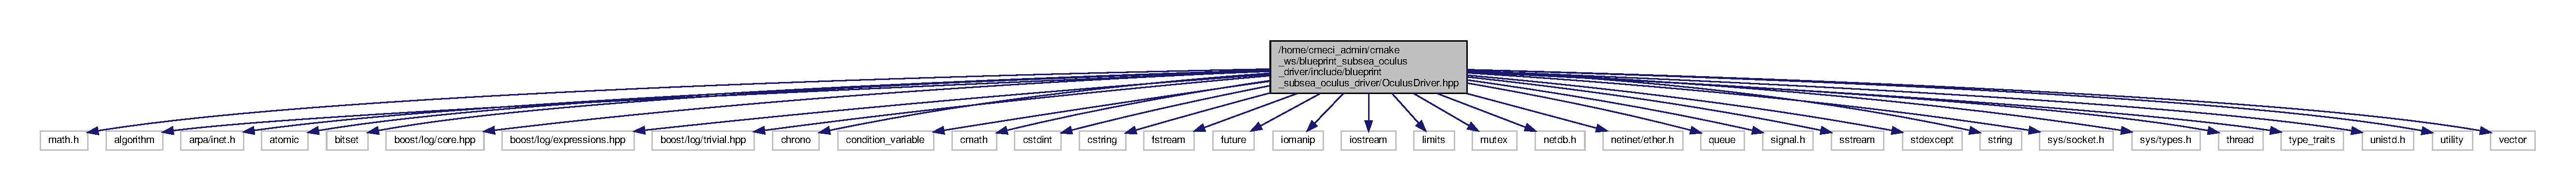
\includegraphics[width=350pt]{OculusDriver_8hpp__incl}
\end{center}
\end{figure}
This graph shows which files directly or indirectly include this file\+:\nopagebreak
\begin{figure}[H]
\begin{center}
\leavevmode
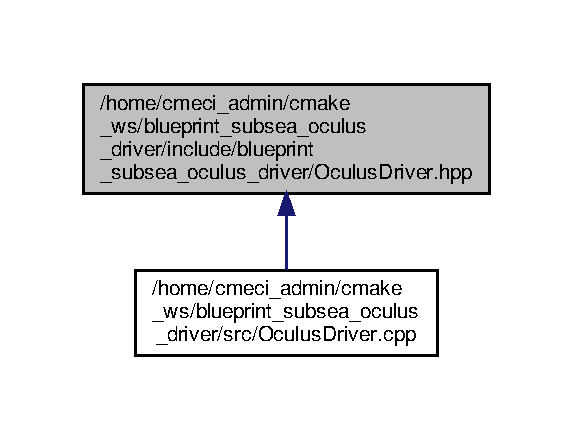
\includegraphics[width=275pt]{OculusDriver_8hpp__dep__incl}
\end{center}
\end{figure}
\subsection*{Classes}
\begin{DoxyCompactItemize}
\item 
class \hyperlink{classOculusDriver}{Oculus\+Driver}
\item 
struct \hyperlink{structOculusDriver_1_1DataPacket}{Oculus\+Driver\+::\+Data\+Packet}
\end{DoxyCompactItemize}


\subsection{Detailed Description}




Copyright 2021 Phil Skelton.

Permission is hereby granted, free of charge, to any person obtaining a copy of this software and associated documentation files (the \char`\"{}\+Software\char`\"{}), to deal in the Software without restriction, including without limitation the rights to use, copy, modify, merge, publish, distribute, sub-\/license, and/or sell copies of the Software, and to permit persons to whom the Software is furnished to do so, subject to the following conditions\+:

The above copyright notice and this permission notice shall be included in all copies or substantial portions of the Software.

T\+HE S\+O\+F\+T\+W\+A\+RE IS P\+R\+O\+V\+I\+D\+ED \char`\"{}\+A\+S I\+S\char`\"{}, W\+I\+T\+H\+O\+UT W\+A\+R\+R\+A\+N\+TY OF A\+NY K\+I\+ND, E\+X\+P\+R\+E\+SS OR I\+M\+P\+L\+I\+ED, I\+N\+C\+L\+U\+D\+I\+NG B\+UT N\+OT L\+I\+M\+I\+T\+ED TO T\+HE W\+A\+R\+R\+A\+N\+T\+I\+ES OF M\+E\+R\+C\+H\+A\+N\+T\+A\+B\+I\+L\+I\+TY, F\+I\+T\+N\+E\+SS F\+OR A P\+A\+R\+T\+I\+C\+U\+L\+AR P\+U\+R\+P\+O\+SE A\+ND N\+O\+N\+I\+N\+F\+R\+I\+N\+G\+E\+M\+E\+NT. IN NO E\+V\+E\+NT S\+H\+A\+LL T\+HE A\+U\+T\+H\+O\+RS OR C\+O\+P\+Y\+R\+I\+G\+HT H\+O\+L\+D\+E\+RS BE L\+I\+A\+B\+LE F\+OR A\+NY C\+L\+A\+IM, D\+A\+M\+A\+G\+ES OR O\+T\+H\+ER L\+I\+A\+B\+I\+L\+I\+TY, W\+H\+E\+T\+H\+ER IN AN A\+C\+T\+I\+ON OF C\+O\+N\+T\+R\+A\+CT, T\+O\+RT OR O\+T\+H\+E\+R\+W\+I\+SE, A\+R\+I\+S\+I\+NG F\+R\+OM, O\+UT OF OR IN C\+O\+N\+N\+E\+C\+T\+I\+ON W\+I\+TH T\+HE S\+O\+F\+T\+W\+A\+RE OR T\+HE U\+SE OR O\+T\+H\+ER D\+E\+A\+L\+I\+N\+GS IN T\+HE S\+O\+F\+T\+W\+A\+RE. 

 
\hypertarget{OculusDriver_8cpp}{}\section{/home/cmeci\+\_\+admin/cmake\+\_\+ws/blueprint\+\_\+subsea\+\_\+oculus\+\_\+driver/src/\+Oculus\+Driver.cpp File Reference}
\label{OculusDriver_8cpp}\index{/home/cmeci\+\_\+admin/cmake\+\_\+ws/blueprint\+\_\+subsea\+\_\+oculus\+\_\+driver/src/\+Oculus\+Driver.\+cpp@{/home/cmeci\+\_\+admin/cmake\+\_\+ws/blueprint\+\_\+subsea\+\_\+oculus\+\_\+driver/src/\+Oculus\+Driver.\+cpp}}
{\ttfamily \#include \char`\"{}blueprint\+\_\+subsea\+\_\+oculus\+\_\+driver/\+Oculus\+Driver.\+hpp\char`\"{}}\newline
Include dependency graph for Oculus\+Driver.\+cpp\+:\nopagebreak
\begin{figure}[H]
\begin{center}
\leavevmode
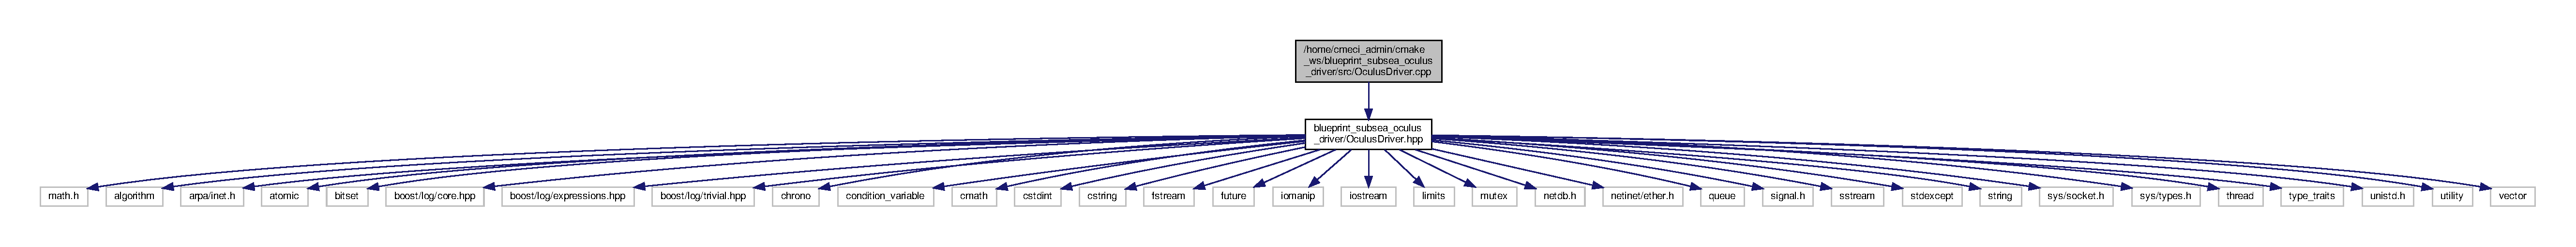
\includegraphics[width=350pt]{OculusDriver_8cpp__incl}
\end{center}
\end{figure}


\subsection{Detailed Description}




Copyright 2021 -\/ Flinders University, Dr Phil Skelton.

Permission is hereby granted, free of charge, to any person obtaining a copy of this software and associated documentation files (the \char`\"{}\+Software\char`\"{}), to deal in the Software without restriction, including without limitation the rights to use, copy, modify, merge, publish, distribute, sub-\/license, and/or sell copies of the Software, and to permit persons to whom the Software is furnished to do so, subject to the following conditions\+:

The above copyright notice and this permission notice shall be included in all copies or substantial portions of the Software.

T\+HE S\+O\+F\+T\+W\+A\+RE IS P\+R\+O\+V\+I\+D\+ED \char`\"{}\+A\+S I\+S\char`\"{}, W\+I\+T\+H\+O\+UT W\+A\+R\+R\+A\+N\+TY OF A\+NY K\+I\+ND, E\+X\+P\+R\+E\+SS OR I\+M\+P\+L\+I\+ED, I\+N\+C\+L\+U\+D\+I\+NG B\+UT N\+OT L\+I\+M\+I\+T\+ED TO T\+HE W\+A\+R\+R\+A\+N\+T\+I\+ES OF M\+E\+R\+C\+H\+A\+N\+T\+A\+B\+I\+L\+I\+TY, F\+I\+T\+N\+E\+SS F\+OR A P\+A\+R\+T\+I\+C\+U\+L\+AR P\+U\+R\+P\+O\+SE A\+ND N\+O\+N\+I\+N\+F\+R\+I\+N\+G\+E\+M\+E\+NT. IN NO E\+V\+E\+NT S\+H\+A\+LL T\+HE A\+U\+T\+H\+O\+RS OR C\+O\+P\+Y\+R\+I\+G\+HT H\+O\+L\+D\+E\+RS BE L\+I\+A\+B\+LE F\+OR A\+NY C\+L\+A\+IM, D\+A\+M\+A\+G\+ES OR O\+T\+H\+ER L\+I\+A\+B\+I\+L\+I\+TY, W\+H\+E\+T\+H\+ER IN AN A\+C\+T\+I\+ON OF C\+O\+N\+T\+R\+A\+CT, T\+O\+RT OR O\+T\+H\+E\+R\+W\+I\+SE, A\+R\+I\+S\+I\+NG F\+R\+OM, O\+UT OF OR IN C\+O\+N\+N\+E\+C\+T\+I\+ON W\+I\+TH T\+HE S\+O\+F\+T\+W\+A\+RE OR T\+HE U\+SE OR O\+T\+H\+ER D\+E\+A\+L\+I\+N\+GS IN T\+HE S\+O\+F\+T\+W\+A\+RE. 

 
%--- End generated contents ---

% Index
\backmatter
\newpage
\phantomsection
\clearemptydoublepage
\addcontentsline{toc}{chapter}{Index}
\printindex

\end{document}
